\section{Метод №2}\label{meth2}

\subsection{Идея}\label{math2:idea}

\begin{itemize}
	\item[1)] Выделяем сетку из всех значений координаты $z$ всех точек трех множеств.
	\item[2)] В каждом множестве добавляем точки с теми $z$, которые присутствуют в сетке, но отсутствуют в текущем множестве: эти точки добавляются на отрезки, соединяющие две ближашие точки множества. Таким образом, получаем разбиение точек трех множеств по "слоям".
	\item[3)] В каждом слое проводим прямые из точек, параллельные направлениям проектирования, и получаем некоторый треугольник. Находим точку, минимально удаленную от трех данных прямых.
	\item[4)] Аппроксимируем полученное множество точек прямой. 
\end{itemize}

\begin{center}
	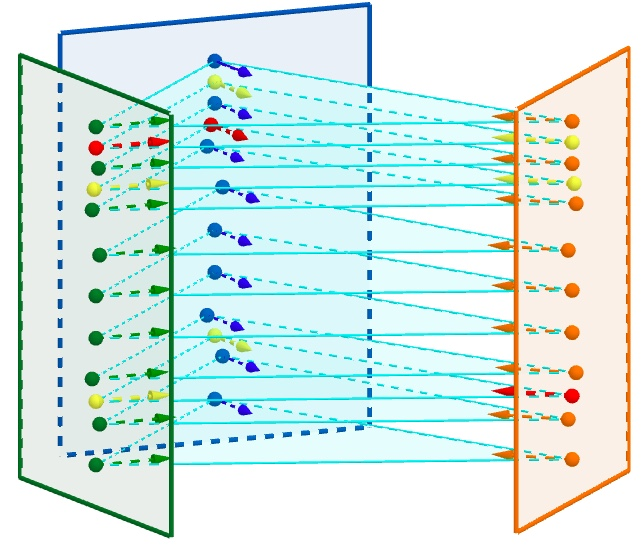
\includegraphics[scale=0.7]{120}

	Рис. 2.2: Добавление точек и разбивка по слоям.

	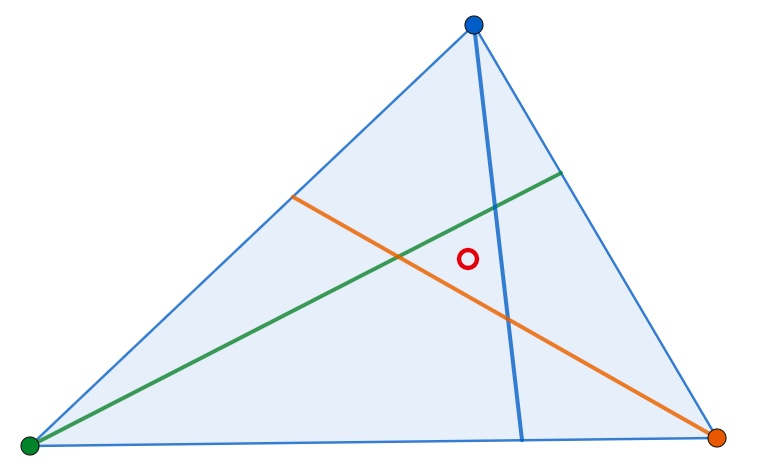
\includegraphics[scale=0.7]{122}

	Рис. 2.3: Нахождение точки, наименее удаленной от данных прямых.
\end{center}

\subsection{Решение}\label{math2:solution}

Алгоритм состоит в множественном применении алгоритма нахождении точки \ref{plane:alg:2dim} в каждом слое, минимально удаленных от проведенных прямых. После этого применяем алгоритм аппрокисимации множества полученных точек прямой \ref{line:alg:3dim}.

\subsection{Погрешность и примеры работы программ}\label{math2:error}

Погрешность складывается из погрешности добавления точек, погрешности множественного применения нахождения точек, минимально удаленных от прямых, и погрешности аппроксимации полученных точек прямой.\\

\newpage
\subsubsection{Искусственные данные}\label{math2:error:synth}

Исходные данные - три множетсва точек и три направления проектирования:

\begin{verbatim}
	(2, -4, 0)	          (-4, 2, 0)            (6.242641, 6.242641, 0)
	(2.1, -4, 1)         (-4, 2.1, 1)          (6.342641, 6.142641, 1)
	(1.9, -4, 2)         (-4, 1.9, 2)          (6.242641, 6.242641, 1.5)
	(2, -4, 3)           (-4, 2, 3)            (6.142641, 6.342641, 2)
	(2, -4, 4)           (-4, 2, 4)            (6.242641, 6.242641, 3)
	(2.1, -4, 5)         (-4, 2.1, 5)          (6.242641, 6.242641, 4)
	(1.9, -4, 6)         (-4, 1.9, 6)          (6.342641, 6.142641, 5)
	(2, -4, 7)           (-4, 2, 6.5)          (6.142641, 6.342641, 6)
	(2, -4, 7.5)         (-4, 2, 7)            (6.242641, 6.242641, 7)
	(2, -4, 8)           (-4, 2, 8)            (6.242641, 6.242641, 8)

	(0, 1, 0)            (1, 0, 0)             (-0.707107, -0.707107, 0)
\end{verbatim}

Полученные данные - направляющий вектор прямой, точка прямой и значение функционала:

\begin{verbatim}
	l = (-0.004403, -0.001467, 1.000000)
	p = (1.999266, 2.000773, 4.291667)
	Lambda = 0.006596
\end{verbatim}

\begin{center}
	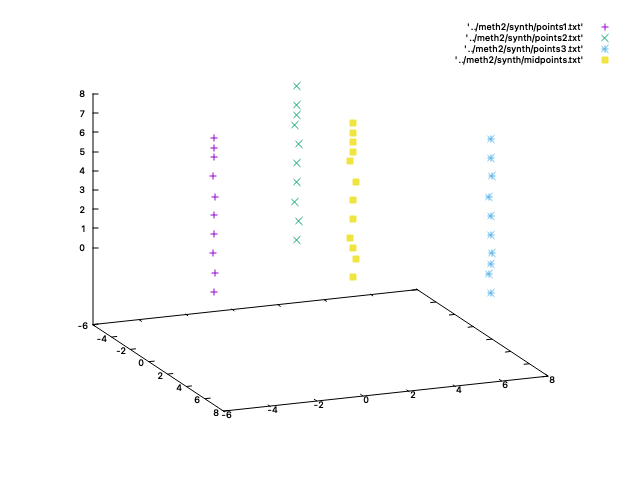
\includegraphics[scale=0.65]{meth2synthmidpoints}

	\textit{<<средние>> точки в каждом слое и исходные множества}

	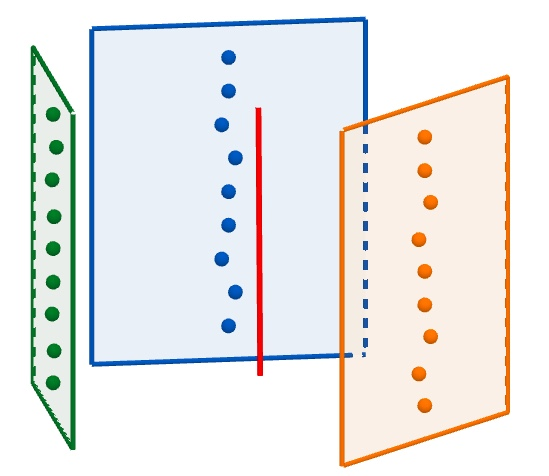
\includegraphics[scale=0.7]{meth2synth}

	\textit{полученный отрезок и исходные множества}
\end{center}

\subsubsection{Реальные данные}\label{math2:error:real}

Исходные данные - 100 множетсв точек и 100 направлений проектирования отрезка, ограниченного по $z$ значениями $-6.08332812434530$ и $-4.57712089734895$. Фигура симметричная, поэтому имеем два искомых отрезка.\\

Полученные данные - по две точки искомых прямых и значения функционала:

\begin{verbatim}
			DATA FOR POSITIVE SET:
	(3.227402, 2.584165, -6.083328)
	(2.505786, 1.505411, -4.577121)
	Lambda = 0.007525
			DATA FOR NEGATIVE SET:
	(-2.979351, -2.779962, -6.083328)
	(-2.377752, -1.727015, -4.577121)
	Lambda = 0.000030
\end{verbatim}

\begin{center}
	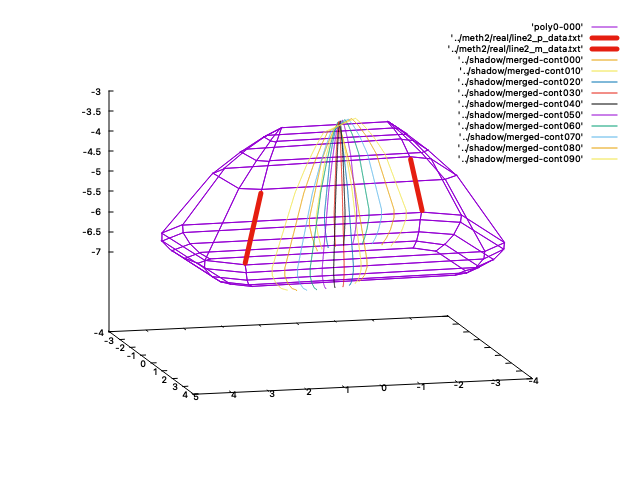
\includegraphics[scale=0.7]{meth2real}

	\textit{искомые отрезки, идеальный контур фигуры и исходные контуры проекций}

	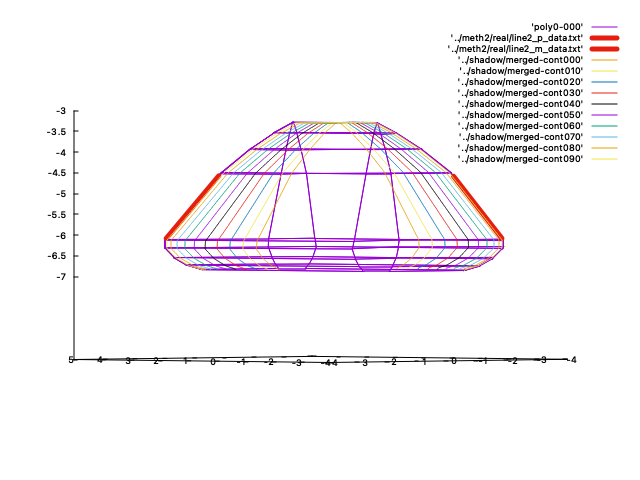
\includegraphics[scale=0.7]{meth2realsideview}

	\textit{искомые отрезки, идеальный контур фигуры и исходные контуры проекций}
\end{center}

\newpage